\documentclass[12pt]{article}\usepackage[]{graphicx}\usepackage[]{color}
%% maxwidth is the original width if it is less than linewidth
%% otherwise use linewidth (to make sure the graphics do not exceed the margin)
\makeatletter
\def\maxwidth{ %
  \ifdim\Gin@nat@width>\linewidth
    \linewidth
  \else
    \Gin@nat@width
  \fi
}
\makeatother

\definecolor{fgcolor}{rgb}{0.345, 0.345, 0.345}
\newcommand{\hlnum}[1]{\textcolor[rgb]{0.686,0.059,0.569}{#1}}%
\newcommand{\hlstr}[1]{\textcolor[rgb]{0.192,0.494,0.8}{#1}}%
\newcommand{\hlcom}[1]{\textcolor[rgb]{0.678,0.584,0.686}{\textit{#1}}}%
\newcommand{\hlopt}[1]{\textcolor[rgb]{0,0,0}{#1}}%
\newcommand{\hlstd}[1]{\textcolor[rgb]{0.345,0.345,0.345}{#1}}%
\newcommand{\hlkwa}[1]{\textcolor[rgb]{0.161,0.373,0.58}{\textbf{#1}}}%
\newcommand{\hlkwb}[1]{\textcolor[rgb]{0.69,0.353,0.396}{#1}}%
\newcommand{\hlkwc}[1]{\textcolor[rgb]{0.333,0.667,0.333}{#1}}%
\newcommand{\hlkwd}[1]{\textcolor[rgb]{0.737,0.353,0.396}{\textbf{#1}}}%
\let\hlipl\hlkwb

\usepackage{framed}
\makeatletter
\newenvironment{kframe}{%
 \def\at@end@of@kframe{}%
 \ifinner\ifhmode%
  \def\at@end@of@kframe{\end{minipage}}%
  \begin{minipage}{\columnwidth}%
 \fi\fi%
 \def\FrameCommand##1{\hskip\@totalleftmargin \hskip-\fboxsep
 \colorbox{shadecolor}{##1}\hskip-\fboxsep
     % There is no \\@totalrightmargin, so:
     \hskip-\linewidth \hskip-\@totalleftmargin \hskip\columnwidth}%
 \MakeFramed {\advance\hsize-\width
   \@totalleftmargin\z@ \linewidth\hsize
   \@setminipage}}%
 {\par\unskip\endMakeFramed%
 \at@end@of@kframe}
\makeatother

\definecolor{shadecolor}{rgb}{.97, .97, .97}
\definecolor{messagecolor}{rgb}{0, 0, 0}
\definecolor{warningcolor}{rgb}{1, 0, 1}
\definecolor{errorcolor}{rgb}{1, 0, 0}
\newenvironment{knitrout}{}{} % an empty environment to be redefined in TeX

\usepackage{alltt}
\usepackage[letterpaper, margin=1in]{geometry}
\usepackage{amsmath}
\usepackage{amsfonts}
\usepackage{amssymb}
\usepackage{mathtools}
\usepackage{graphicx}
\usepackage{indentfirst}
\usepackage{hyperref}
\UseRawInputEncoding
\pagenumbering{gobble}
\pagenumbering{arabic}
\usepackage{verbatim}
\usepackage{setspace}
\immediate\write18{texcount -tex -sum  \jobname.tex > \jobname.wordcount.tex}

% Keywords command
\providecommand{\keywords}[1]
{
  \small	
  \textbf{\textit{Keywords---}} #1
}

%PREAMBLE
\title{The Federal Reserve's LSAP Program: A Predictive Approach Post the 2008 Financial Crisis}
\author{Ivan Lozano\thanks{MSc Applied Economics, Boston College, 140 Commonwealth Avenue, Chestnut Hill, MA 02467, lozano037@gmail.com}\\} 
\date{\small April 13, 2023}

%CONTENT
\IfFileExists{upquote.sty}{\usepackage{upquote}}{}
\begin{document}
\begin{singlespace}

\maketitle

\begin{abstract}
The objective of this paper is to address the impact the financial crises of 2008 had on the housing market and what the average prices of homes will look like in the future. Data is obtained from the Federal Reserve Economic Database (FRED) for Mortgage-Backed Securities and Treasuries bought and sold by the Federal Reserve. Constant long-term treasuries from FRED are compiled as well. Data for real home prices was obtained from Case-Shiller, which are two economists who gather data of monthly home values. Mortgage rate data is gathered from Freddie Mac, which is a Government-Sponsored enterprise that shows how mortgage rates fluctuate over time for 30-year and 15-year maturities. Finally, we added the purchasing manager's index, which is made up of the aggregate number of new capital goods orders and percent change in non-farm payrolls. This paper explains how average home prices will fluctuate in the next six months using the effects of interest rates and asset purchases through regressive techniques. Ultimately, this paper finds that since July of 2009, the Federal Reserve's action in buying mortgage-backed securities increased the real house price index by 6.2 percent for every 1\% increase in MBS purchases. In our forecasting analysis, this paper shows that the Seasonal Naive and the Neural Network Autoregression are the best methods for predicting the housing price index.

\keywords forecasting, house prices, mortgage-backed securities, treasuries, machine learning


\end{abstract} \hspace{10pt}
\end{singlespace}
\newpage

\doublespacing
\section{Introduction}

The 2007-2009 financial collapse was one of the worst recessions in the US and also a global meltdown. The recession was caused by multiple factors, including the failure of the US financial system, the housing market, and unregulated markets. The US government and the Federal Reserve System were key players in assisting the economy to recover through the use of fiscal and monetary policy. The government provided investment bank and insurance bailouts, passed by Congress, to reduce the negative externalities of smaller bank failures that were owned by larger banks. On the monetary policy side, the Federal Reserve enacted a quantitative easing program, where it used its monetary power to buy up Mortgage-Backed Securities (MBS) and Treasuries to assist the economy in slowing down. MBS products largely fell in price within seconds during the financial crisis, and large investment banks owned many of these risky assets. The goal of the quantitative easing program was to pump liquidity or cash into the market and assist investment banks from bankruptcy. The other main objective of this policy was to reduce the Federal Funds Rate, or better known as the overnight lending rate, to keep the economy moving after the housing market experienced significant losses in home values. The Federal Reserve's dual mandate of keeping inflation stable and low unemployment during the housing market crash had several positive effects to help the US economy recover.

\par
One role where the Federal government intervened before the financial collapse in 2008 was increased government spending in Government Sponsored Entities, or GSE's for short. The main GSE's are Fannie Mae, Freddie Mac, and Ginnie Mae. The main goal of GSE's was to increase the availability of credit in the housing market. GSE's displayed a significant role in the failure of the financial system as it guaranteed the underlying loans behind MBS products. MBS products are financial instruments compiled of underlying home mortgage loans that are packaged by investment banks and sold to investors.

\par
The combination of fiscal policy and monetary policy has historically impacted the economy measured by the labor market, GDP growth, and inflation. The goal of this research will be to take a time-series econometric approach into how large-scale asset purchase program (LSAP) action by the Federal Reserve affected national housing prices and I will explain how LSAP caused ripple effects on mortgage rates and treasury rates. The data being used will be from the St. Louis Federal Reserve Economic Database (FRED), Case-Schiller Housing Price Index, Bureau of Labor Statistics, Freddie Mac interest rates and the Institute Supply of Management. I will observe mortgage rates, real housing prices, treasury rates, non-farm payrolls, and the purchasing manager's index. Through this research I will train models through predictive analytics to measure changes due to the Federal Reserve's LSAP initiative. Models include time-series multivariate regressions which include the real house price index as our response variable, with the percent difference in mortgage-backed securities bought and sold by the Federal Reserve. The models control for non-farm payroll percentage growth change, purchasing manager's index (PMI) difference, and interest rates. Data is aggregated on a monthly basis since 2017, which is when the Federal Reserve began showing activity in their balance sheet of MBS products. Forecasting method's will include our multi-variate time-series model along with random walk, mean, naive, arima, seasonal naive and neural network forecasting.

\section{Hypothesis}

\emph{Hypothesis I}: The purchases of mortgage-backed securities by the Federal Reserve inflated the average home prices measured by the difference in real home price index.

\emph{Hypothesis II}: The reduction in the constant 10-year treasury rate has increased the national average of US home prices, measured by the difference in real home price index.

\section{Literature Review}

\par 
Prior research on the effects of this large scale asset purchase (LSAP) by the Federal Reserve has been researched, and findings have shown to have direct effects on interest rate as intended, but also the value of housing in the nation. Research that I have found stems mainly from the Federal Reserve System, the Urban Institute, the Bureau of Labor Statistics, Stanford University, the University of California at Berkeley, and Cornell University.
\par
The first source, I want to touch base upon is the Finance and Economics Discussion Series by the Federal Reserve Board, ``Did the Federal Reserve's MBS Purchase Program Lower Mortgage Rates?'', which aims to identify risk premiums that were embedded in mortgage and swap markets. In summary, their goal is to understand the differences between the MBS purchase program's effect in lowering mortgage rates. The authors suggest, "around half of the declines in risk premiums that were associated with improved market functioning and about half with the declines in risk premiums that were associated with changes in the compensation for holding fixed-rate financial assets over a long period", showing the MBS program has a direct effect on market functionality in holding fixed-rate assets over a longer period on their balance sheet (Hancock and Passmore 2011). Hancock et. al. mention that their results are not fully conclusive, but it shows that further research could be useful in showing more robust results. Another academic article on the MBS purchase program is written by Stroebel and Taylor. They intend to identify the impact of quantitative easing, or the large-scale asset purchase (LSAP) had on the level of mortgage spreads. The results show a statistically significant effect on mortgage spreads of about 30 basis points, which can be found as a measure of option-adjusted based on the treasury yield curve (Stroebel and Taylor 2012). Although they state that it has no effect on the existence of the program, this will portray similar or slightly different effects based on our analysis of mortgage spreads impact on the housing market. While it is important to show the effective influence that QE had on the housing market, authors have explained that it is a difficult task to measure the level of change in mortgages.
\par
Another perspective of the effect how the LSAP program by the Federal Reserve may have had on the housing market has been analyzed by Geoffrey Paulin who works at the Bureau of Labor Statistics where he aims to show changes in the median and average home sale price decreases during the recession. He describes the shifts in homeownership rates by region in the United States, noting a sharp increase in the western region, but overall most US regions had noticeably lower homeownership rates in 2015 as opposed to before 2008 (Paulin 2018). This article explains more of a summary of statistics on how homeownership and median and average prices of homes changed during and after the recession and it is important to get an idea of the macroeconomic effects of how the LSAP program may have influenced the valuation of housing prices by region. This article also states the effect of the housing bubble concerning the renter's market, he notes, ``there is evidence of a post-bubble effect: from 2007-2009, rents in rural areas declined substantially, to levels not seen since 2003'', which denotes a large difference from urban areas rental expenditure compared to rural areas. The Urban Institute explains the motives for the Federal Reserve's traditional tools for stimulating the economy being insufficient, thus engaging in buying Mortgage-backed securities from the private sector to further help the economy from the crisis (Goodman and Bai 2017). This paper's goal is to analyze the motives for the Federal Reserve's decisions to affect the housing market. The authors note the Federal Reserve owns about 28 percent of the mortgage market. This explains the significance of how changes in their balance sheet historically have affected the mortgage market, but the reverse effect can occur if the Federal Reserve decides to sell the MBS and Long-Term Treasury products. Lastly, Plakandaras et. al. shows how housing prices through adverse macroeconomic conditions can be used as a predictor in measuring sudden drops in the housing market. The authors conclude that using Bayesian autoregressive forecasting methodology, using 11 other independent variables, can be used as an effective policy instrument for determining the business cycle in the economy (Plakandaras et. al. 2017). In my analysis, I will show the changes in the real housing prices per the buying of fixed-rate treasuries through the LSAP program using different time-series econometric approaches.
\par
Overall, researchers have shown the LSAP program had positive effects on financial markets and lowered the level of interest rate changes related to the housing market during the 2008 financial crisis. The goal of the Federal Reserve's program was to help the economy recover from its high rates of unemployment, which was directly caused by the housing collapse, it is important to closely observe the changes in the housing market to avoid another disruption in the economy. In another paper, the Kansas City Federal Reserve explains how asset prices are likely to be affected by treasury yields, inflation swaps, corporate bonds, and agency MBS prices regarding different points in the quantitative easing timeline (Krishnamurthy and Vissing-Jorgensen 2013). Relative to option-adjusted treasury spreads during the period of QE, there is a reduction in secondary market production of MBS products. The author goes on to state, ``the yield on the production [of] MBS is an important factor in determining the cost to a bank of making a new agency-securitizable mortgage loan''. They conclude by restating the importance of the spillover effects of LSAPs. In specific, outlining how MBS has more of an effect on the private sector than treasuries. This portrays some evidence that the large-scale asset purchase program of MBS products by the Federal Reserve is likely to affect the private sector. In my analysis, I will show the effects of the housing market in proportion to the MBS purchases made by the Federal Reserve.

\section{Data and Methodology}
Data is collected from the Federal Reserve Economic Data (FRED) online database and will show the change of securities held by the Federal Reserve over time, which they began buying on January 14, 2009. Mortgage-backed securities and treasuries held by the Federal Reserve extracted from FRED. Based on the latest statistical release by the Fed, a large portion of MBS products is guaranteed by Fannie Mae, Freddie Mac, and Ginnie Mae (Federal Reserve Statistical Release 2019), thus signaling a connection to housing market interest rates. Long-term 10-year constant treasury yields are also from FRED. Total Nonfarm Payrolls in the  originate from the Bureau of Labor Statistics, a measure of the number of US workers in the economy that excludes proprietors, private household employees, unpaid volunteers, farm employees, and the unincorporated self-employed, which accounts for approximately 80\% of the workers contributing to GDP. The secondary source utilized are changes in mortgage rate durations over time gathered from Freddie Mac. As stated before, Freddie Mac was one of the largest GSEs that played a role in the financial crisis of 2008. Observed from the Federal Reserve balance sheet, MBS products are guaranteed by GSEs including Freddie Mac. These were bought in large amounts to stabilize the economy. The real house price index show's the national average price of house prices in the US collected by the Case-Schiller Index. Another macroeconomic indicator included in my modeling is the purchasing manager's index, which shows economic trends in the manufacturing sector. The PMI comes from the Institute for Supply Management and is a survey sent to senior executives at more than 400 companies in 19 industries which are weighted by their contribution to US GDP. The Report monitors activity in production, new orders, supplier deliveries,  inventory, employment prices, imports, and exports. In my analysis, I will show how the Central Bank of the US may have influenced the value and rate changes in the housing market, and to further explain how changes in monetary policy through the LSAP program have influenced the housing price index.

\subsection{Summary Statistics}
The first data set that I want to address is on Mortgage-Backed securities and Treasuries bought and held by the Federal Reserve at the beginning of 2009. The data was extracted from the Federal Reserve Economic Database and includes the weekly purchases since the inception of the quantitative easing program. I will first start by addressing the trends and summary statistics in each of my variables. Appendix A will contain all of the graphs, tables, and charts.

\par
Graph 1 in Appendix A contains the time-series chart of mortgage-backed securities and treasuries held by the Federal Reserve. Before any data cleaning or transformations, we see the Federal Reserve did not start buying MBS products until 2009, thus we will have to eliminate several observations to reduce the skew of our data set. Secondly, since we have weekly observations in this dataset, we will have to aggregate the data by month. This is mainly due to our response variable, HPI, having monthly observations. Initially, we had 848 observations. Graph 2, shows the time-series chart of historical mortgage rates for 30-year and 15-year fixed rates since 1970. We can observe that points where recessions hit the US economy had high rates of mortgage rates, followed by fairly large drops. In Graph 2 from the time plot, we also see the points in time where the recession hits have a large change in mortgage interest rates. This also shows a big change in the 1980s, when a recession occurred. Over time the trend lines are sloping downward aside from the graph, and proper cleaning will need to be conducted to have more accurate forecasting, looking at the before and after effects of the LSAP purchase by the Federal Reserve. During our modeling process, we have also subsetted our data to include observations from July 2009 and which will be later explained in our data cleaning process. Graph 3, displays 10-year constant treasury rates and shows a more stationary graph since 2002.

\par
Moving to our key dependent variable in our study, Graph 4 display's the trend line fluctuations in the real housing prices, nominal housing price index, and consumer price index (CPI) as a measure of inflation. We can observe from this graph a gap between real and nominal HPI. This show's that housing prices are increasing with a higher rate of inflation in the housing market. Furthermore, we can see that peaks and valley of the 2008 financial crisis. Lastly, Graph 5 displays non-farm payrolls, and the purchasing manager's index. These are key independent variables, because they are macroeconomic indicators of how well the US economy is performing in terms of a measure of unemployment rate and manufacturing. We can observe the drop of the 2008 financial crisis in both graphs, but we will need to transform the PMI to get a more stationary dataset.

\par
It is important to note that our data for mortgage-rates also do not have the same time-frame as the housing price index, but we will address this situation in the data cleansing process as well. Initially we observed the number of observations across 4 metrics of mortgage rates ranged from 730 observations to 2492 observations. In our forecasting, the time will be limited to the before and after effects of the 2008 recession, but it is important to understand all of the data collected to get a broad picture of how the economy performs throughout its business cycles. The highest averages from our mortgage rate data is 30-year fixed data.

\par
Now that we have outlined the time plots of our data, we will prepare our data for our forecasting methods. The first tool that we will be using to compare our data is setting up cutoff points in time for a year when the Federal Reserve began buying MBS and treasuries from the financial market through its use of open market operations

\subsection {Data Cleansing}
The data cleaning process involved several steps since the initial datasets contained several zero values, and the time-frequency was different for the datasets collected. The first part is selecting a fair starting point to measure the actual effects of the buying and selling of the Federal Reserve's assets buys and sells. Thus the starting point was set to July 2009 because the Federal Reserve did not begin buying up assets until January 2009 and the first six months involved vary large purchases that skewed our data. Thus, we cut and merged all our data using July of 2009 data.

\par
The next setop in our data cleaning process was to set all our data to the frequency of our response variable, the Housing Price Index (HPI). Since the Case-Schiller Index is aggregated monthly we set this as our time frequency for the rest of our dataset. This required us to aggregate our weekly observations by month. This involved taking the mean average beginning in July of 2009 for mortgage rates, mortgage-backed securities and treasury rates. After we did this we were able to merge another preliminary master dataset.

\par
The third step in our process involved taking the first difference of some of our variables, to obtain a percentage change. This was critical for interpretation, but also to obtain more stationary and normal datasets. For purchasing managers index, and the housing price index we took the first difference. We also took the first difference percentage change of our treasuries and MBS products bought and sold by the Federal Reserve. This was effective in having interpretable regression results and normalizing the data.

\par
After aggregating and merging all of our datasets there were 114 observations in total. The lowest mean of our data was the difference in MBS purchases, but was highly skewed to the left due to the larger initial purchases by the Federal Reserve as shown in Table 1 and Graph 5. This was the same case for treasuries bought and sold by the Federal Reserve. The rest of our independent variables and Real HPI are fairly normally distributed after transforming them.

\subsection{Forecasting Methods}
\par
Using our forecasting methods as a preliminary method, we can populate 4 different type of forecasting tools. The first data set that we use is the 30 year fixed mortgage rates. From our graph we can see that the seasonal na�ve method appears to fit the closest to our charts. Based on the forecasting methods in graphs 6 and 7, we can observe that for the Mortgage data we see that the seasonal na�ve method works best for both the 30-year and 15-year mortgages. As for the forecasting methods of the MBS and Treasuries, we can observe that none of the methods show a strong effect of forecasting. In Graph 6 we observe that mortgage-rates and treasuries are negatively correlated with real house price index. Non-farm payroll's on the other hand are positively related with the real house price index. Graph 7, show's the correlation matrix, so we can numerically see which variables are highly correlated with each other. This is important to avoid multicollinearity with highly correlated explanatory variables. Also, we observe no variables highly correlated with real house price index, thus endogenity is not a high concern, but may still be present depending on our modeling strategy.

\par
Graph 7 show's the first model which included an autoregressive model with only the historical changes in the differenced real house price index. Based on the graph we observe some seasonality and the the height of the peaks, get lower as time progresses after 2013. Our next approach is to create a multivariate regression to come up with better predictions. The first model included MBS differences, PMI, 10-year treasury rates and non-farm payrolls (payems). The result showed that MBS buys and sells since July 2009 had a 10.29 percent increase in real housing price index, and is significant at .001 probability value. The second model included MBS differences, PMI, 30-year mortgage rates and non-farm payrolls (payems). This also showed the MBS differences and 30-year fixed mortgage rates had a significant effect on real housing prices with a 9.88 percent increase. From the residual plots, we can see that the residuals are normally distributed, and the ACF plot show's seasonality in the model. The third model included treasury differences (treas diff), PMI (ism pmi diff), 15 year fixed mortgage rates(yr 15 fixed), and non-farm payrolls (payems). The result show that only 15 year mortgage rates explained for .52 percent decrease in housing price index. The adjusted r-squared was .12, which is important to show that a different approach is valid. Our second model, included the MBS differences, PMI, non-farm payrolls and 30-year mortgage rates. This model performed with less robust results, but ultimately show's that treasuries had a marginal effect on the percent change of real house price index.

\par
The final part of our forecasting methodology was to use predictive models to back test our historical data. In summary, we split the data with an 80-20 percent train and test split. The models performed: drift, mean, na\"ive, neural network autoregression (AR), a combination of neural network AR, and a seasonal na\"ive method. Then we used several parameters to test the accuracy of our model. After, running our diagnostics, of seasonal na\"ive method performed the best with the lowest root-mean squared error of .33 as shown in Table 4. Finally we were able to run the seasonal naive method using our best performing multi-variate time series regression to forecast 24 months into the future. As we can see from our final graph, there appears to be a seasonal change in the percent change of Real HPI with a fairly large standard error at the 80 and 95 confidence interval. Nonetheless, we can observe a pattern.


\section{Conclusion}
\par
Per our hypothesis we wanted to get an understanding the effects of the the large-scale asset purchase program by the Federal Reserve. Ultimately, we found a significant effect of a 6.2 percent increase in the real housing price index ror every 1\% increase in mortgage-backed securities bought by the federal reserve since the 2009 start of the LSAP program. Interestingly enough the seasonal na\"ive method outperformed each of its counter-party forecasting methods in predicting future increases and decreases in the real house price index. From the time-series charts we can observe that there is a clear effect in the trend of the mortgage rates, when the Federal Reserve began buying mortgage-backed securities secured by government sponsored entities. Another conclusion we can draw from the real housing price index is that it experiences seasonality. The housing market experiences slowdowns during the winter months, and is more active during the summer months. The changes in mortgage interest rates could be the opposite effect of the housing cycle. Thus continued research and monitoring of the Feds assets purchases and sells is key to understanding housing market trends.

\newpage
\appendix
\section{\\Appendix A: Tables and Graphs}





\begin{knitrout}
\definecolor{shadecolor}{rgb}{0.969, 0.969, 0.969}\color{fgcolor}
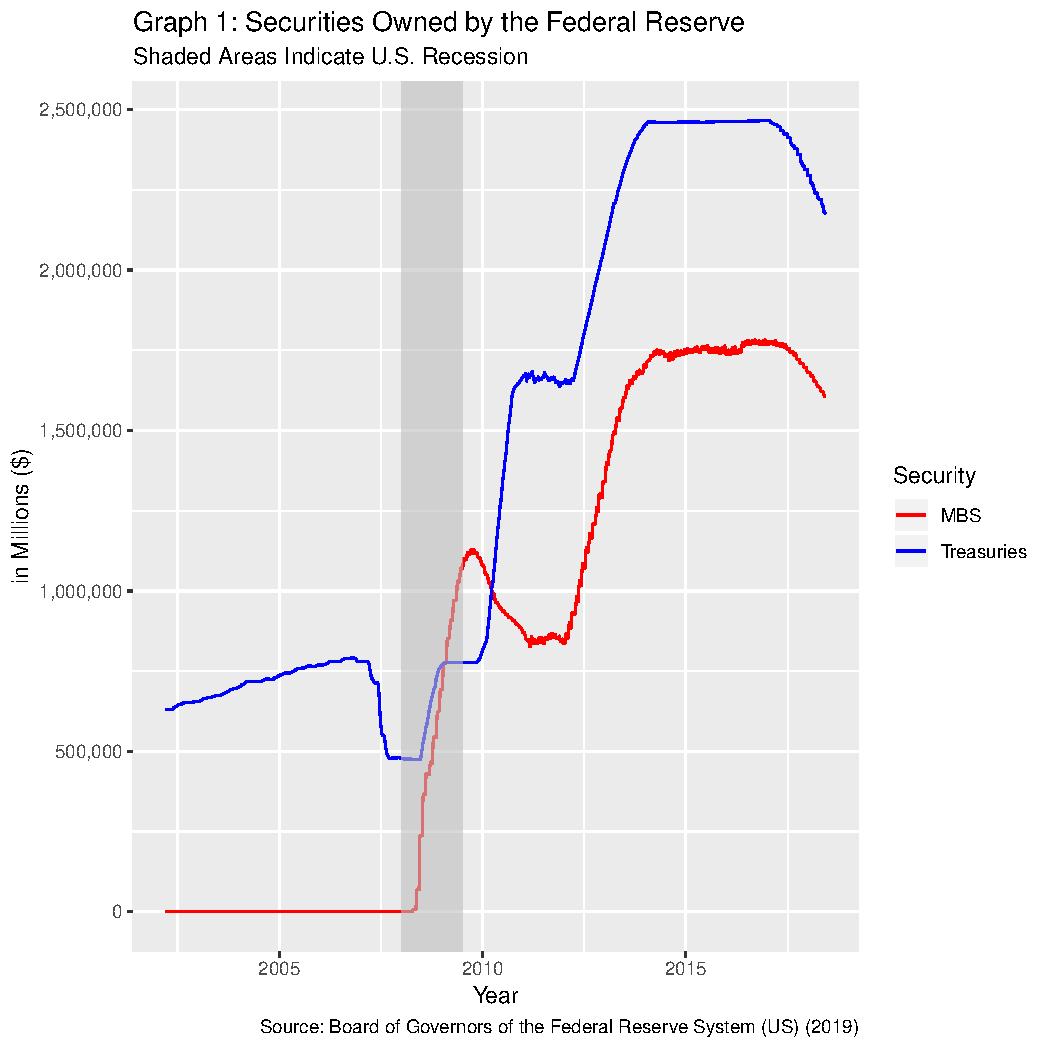
\includegraphics[width=\maxwidth]{figure/unnamed-chunk-2-1} 

\end{knitrout}

\begin{knitrout}
\definecolor{shadecolor}{rgb}{0.969, 0.969, 0.969}\color{fgcolor}
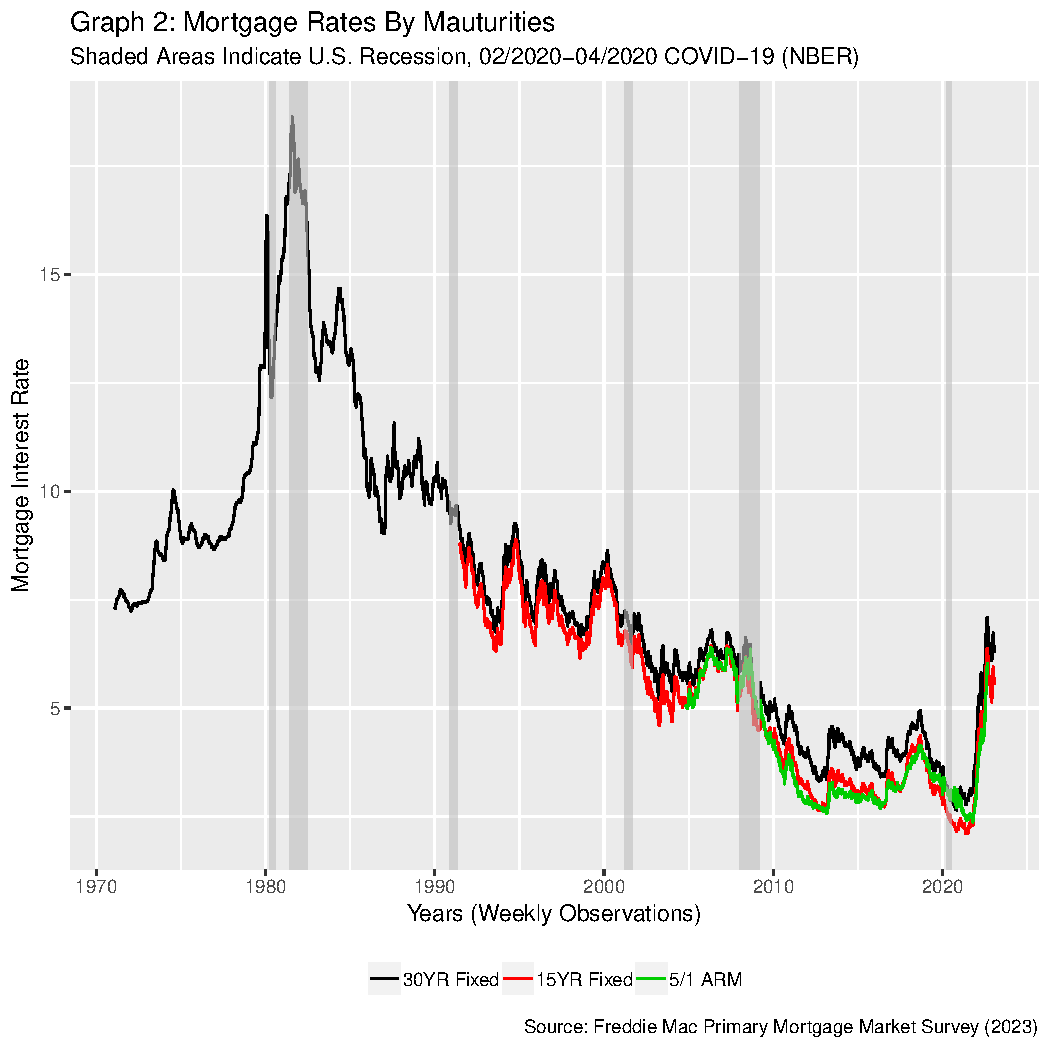
\includegraphics[width=\maxwidth]{figure/unnamed-chunk-3-1} 

\end{knitrout}

\begin{knitrout}
\definecolor{shadecolor}{rgb}{0.969, 0.969, 0.969}\color{fgcolor}
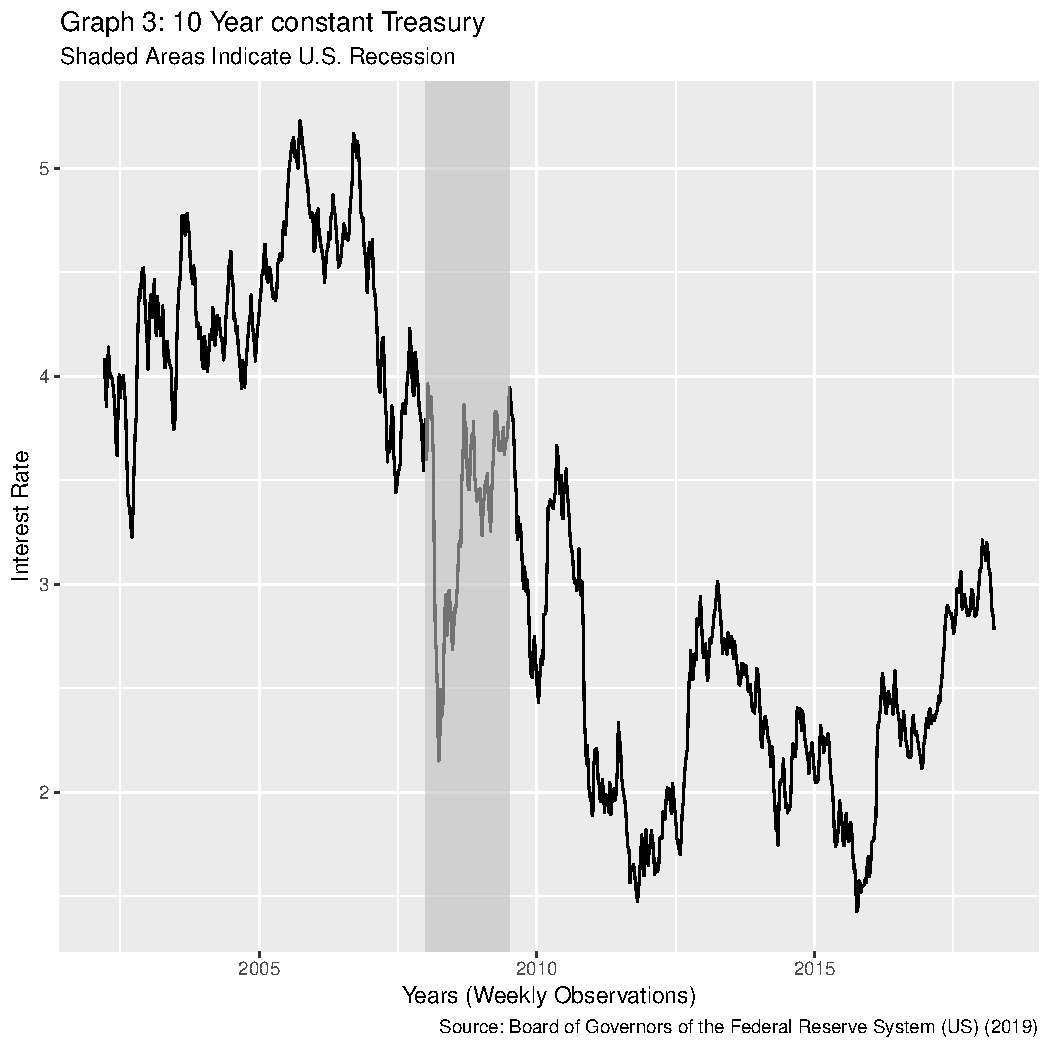
\includegraphics[width=\maxwidth]{figure/unnamed-chunk-4-1} 

\end{knitrout}

\begin{knitrout}
\definecolor{shadecolor}{rgb}{0.969, 0.969, 0.969}\color{fgcolor}
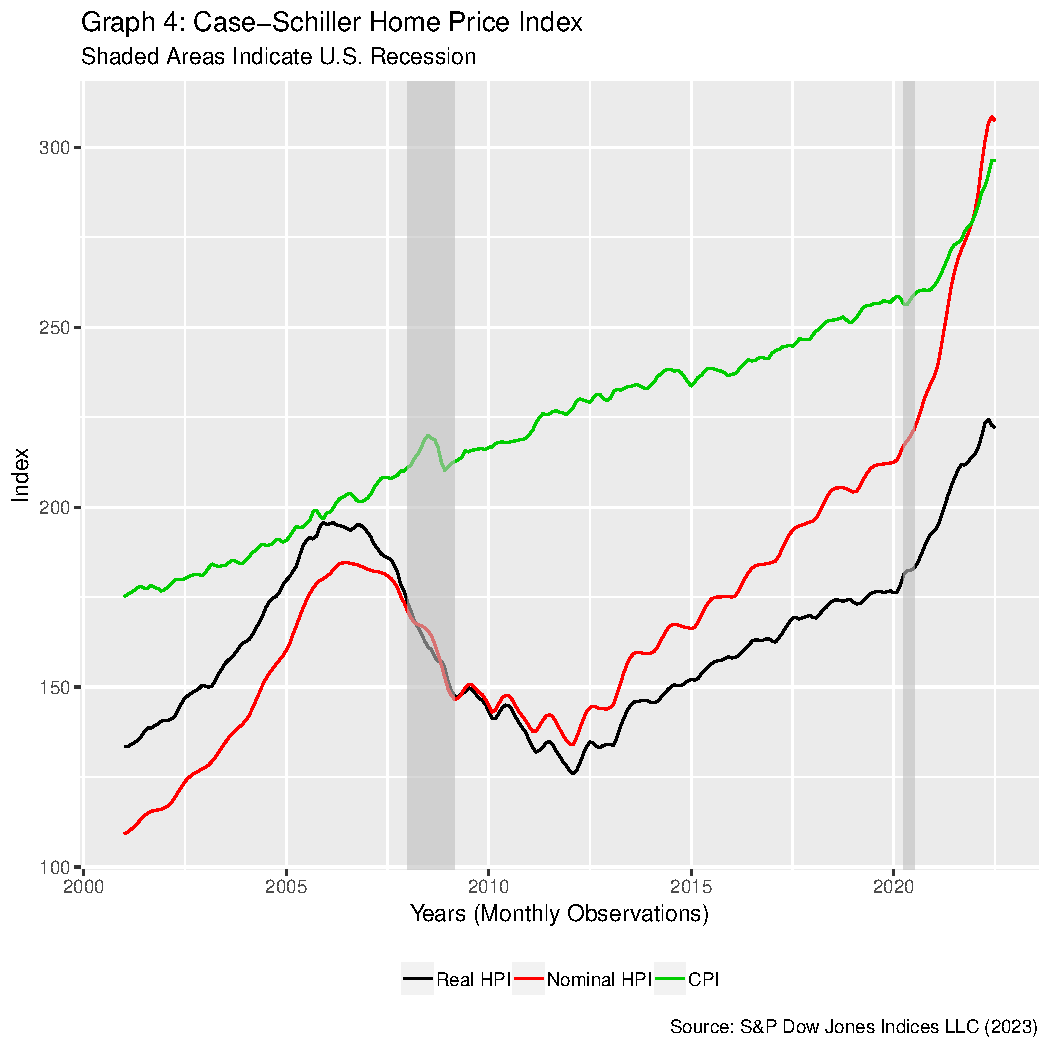
\includegraphics[width=\maxwidth]{figure/unnamed-chunk-5-1} 

\end{knitrout}

\begin{knitrout}
\definecolor{shadecolor}{rgb}{0.969, 0.969, 0.969}\color{fgcolor}
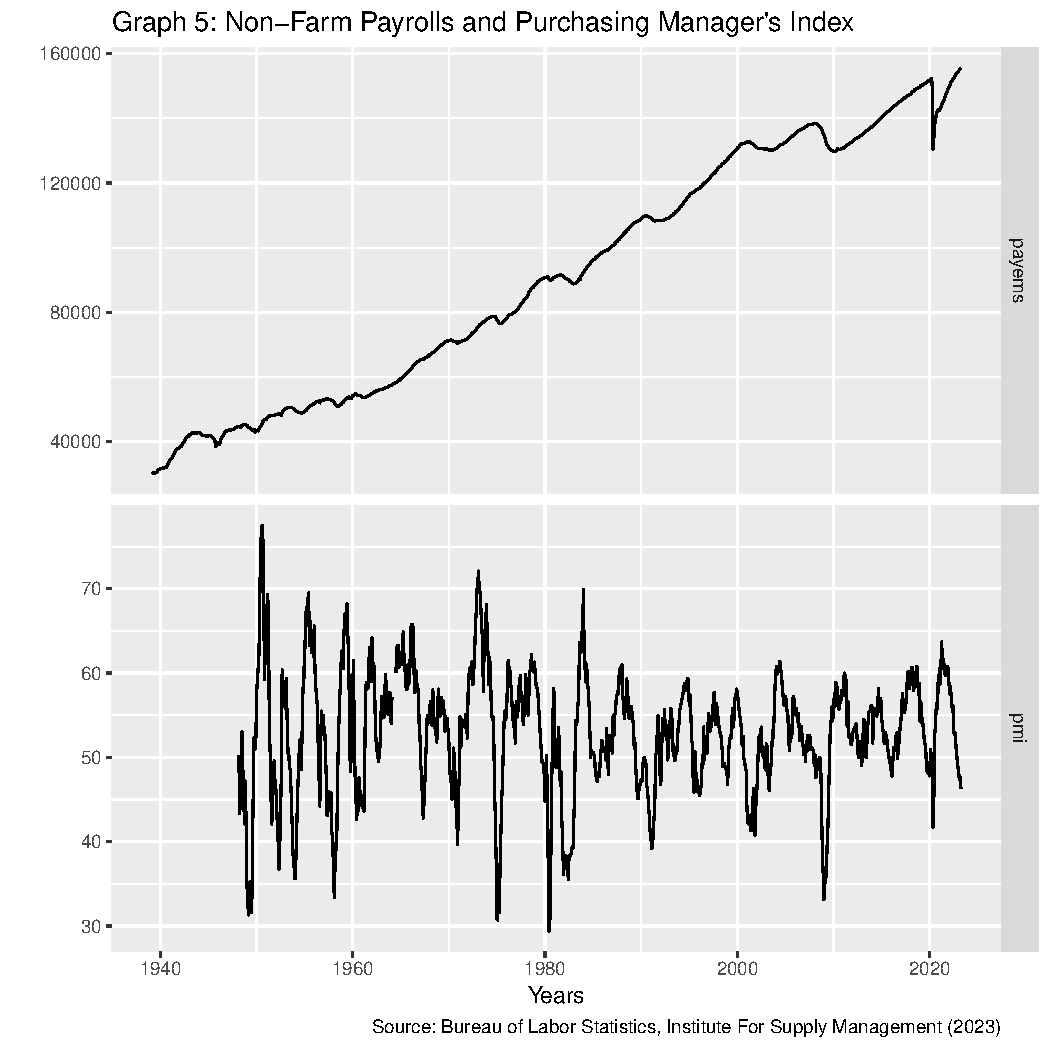
\includegraphics[width=\maxwidth]{figure/Data_and_Methodology-1} 

\end{knitrout}


\begin{knitrout}
\definecolor{shadecolor}{rgb}{0.969, 0.969, 0.969}\color{fgcolor}
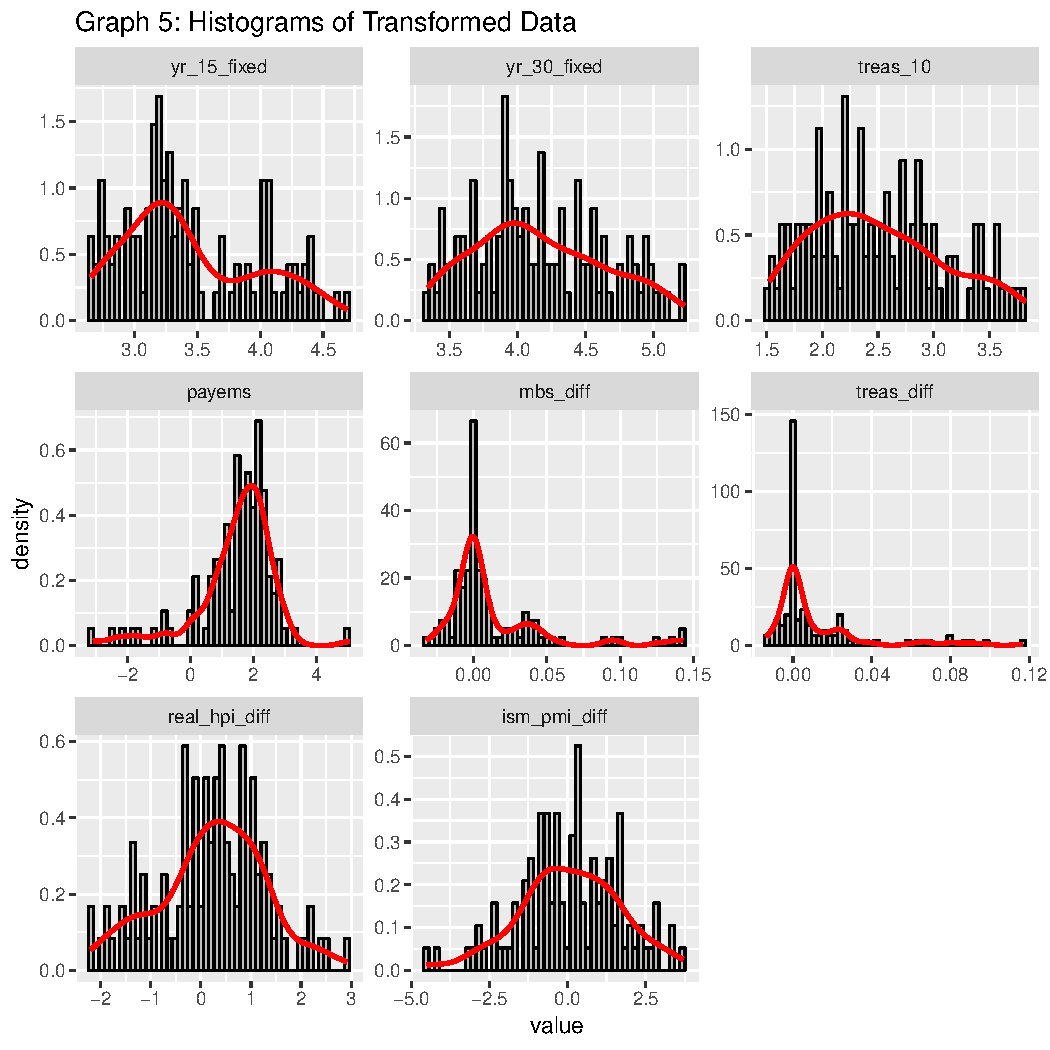
\includegraphics[width=\maxwidth]{figure/unnamed-chunk-6-1} 

\end{knitrout}

\begin{knitrout}
\definecolor{shadecolor}{rgb}{0.969, 0.969, 0.969}\color{fgcolor}\begin{table}[t]

\caption{\label{tab:Descriptive Statistics}Table 1: Summary Statistics}
\begin{tabular}{l|r|r|r|r|r|r|r|r|r|r|r|r|r}
\hline
  & vars & n & mean & sd & median & trimmed & mad & min & max & range & skew & kurtosis & se\\
\hline
yr\_15\_fixed & 1 & 155 & 3.31 & 0.63 & 3.21 & 3.29 & 0.55 & 2.15 & 4.90 & 2.76 & 0.35 & -0.48 & 0.05\\
\hline
yr\_30\_fixed & 2 & 155 & 4.00 & 0.63 & 3.96 & 4.00 & 0.60 & 2.68 & 5.52 & 2.84 & 0.09 & -0.47 & 0.05\\
\hline
mbs\_diff & 3 & 155 & 0.01 & 0.03 & 0.00 & 0.01 & 0.01 & -0.03 & 0.15 & 0.18 & 2.21 & 5.16 & 0.00\\
\hline
treas\_diff & 4 & 155 & 0.02 & 0.04 & 0.00 & 0.01 & 0.01 & -0.03 & 0.40 & 0.43 & 6.27 & 54.55 & 0.00\\
\hline
real\_hpi\_diff & 5 & 155 & 0.48 & 1.19 & 0.45 & 0.47 & 1.10 & -2.20 & 3.67 & 5.87 & 0.05 & -0.17 & 0.10\\
\hline
ism\_pmi\_diff & 6 & 155 & 0.07 & 1.95 & 0.00 & 0.07 & 1.63 & -8.00 & 9.10 & 17.10 & 0.11 & 3.85 & 0.16\\
\hline
payems\_diff & 7 & 155 & 138.77 & 1741.20 & 211.00 & 219.18 & 120.09 & -20514.00 & 4565.00 & 25079.00 & -10.64 & 125.01 & 139.86\\
\hline
\end{tabular}
\end{table}


\end{knitrout}


\begin{knitrout}
\definecolor{shadecolor}{rgb}{0.969, 0.969, 0.969}\color{fgcolor}
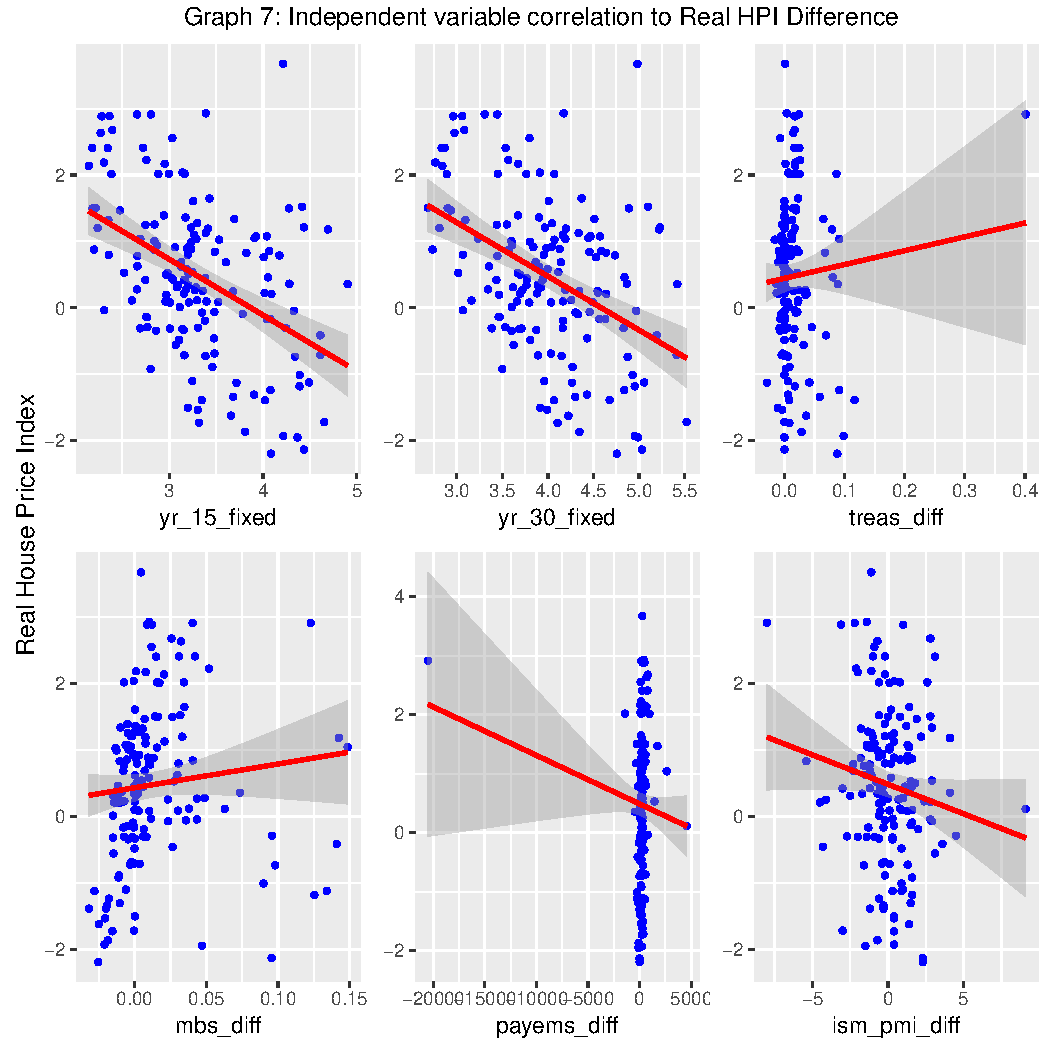
\includegraphics[width=\maxwidth]{figure/unnamed-chunk-7-1} 

\end{knitrout}

\begin{knitrout}
\definecolor{shadecolor}{rgb}{0.969, 0.969, 0.969}\color{fgcolor}
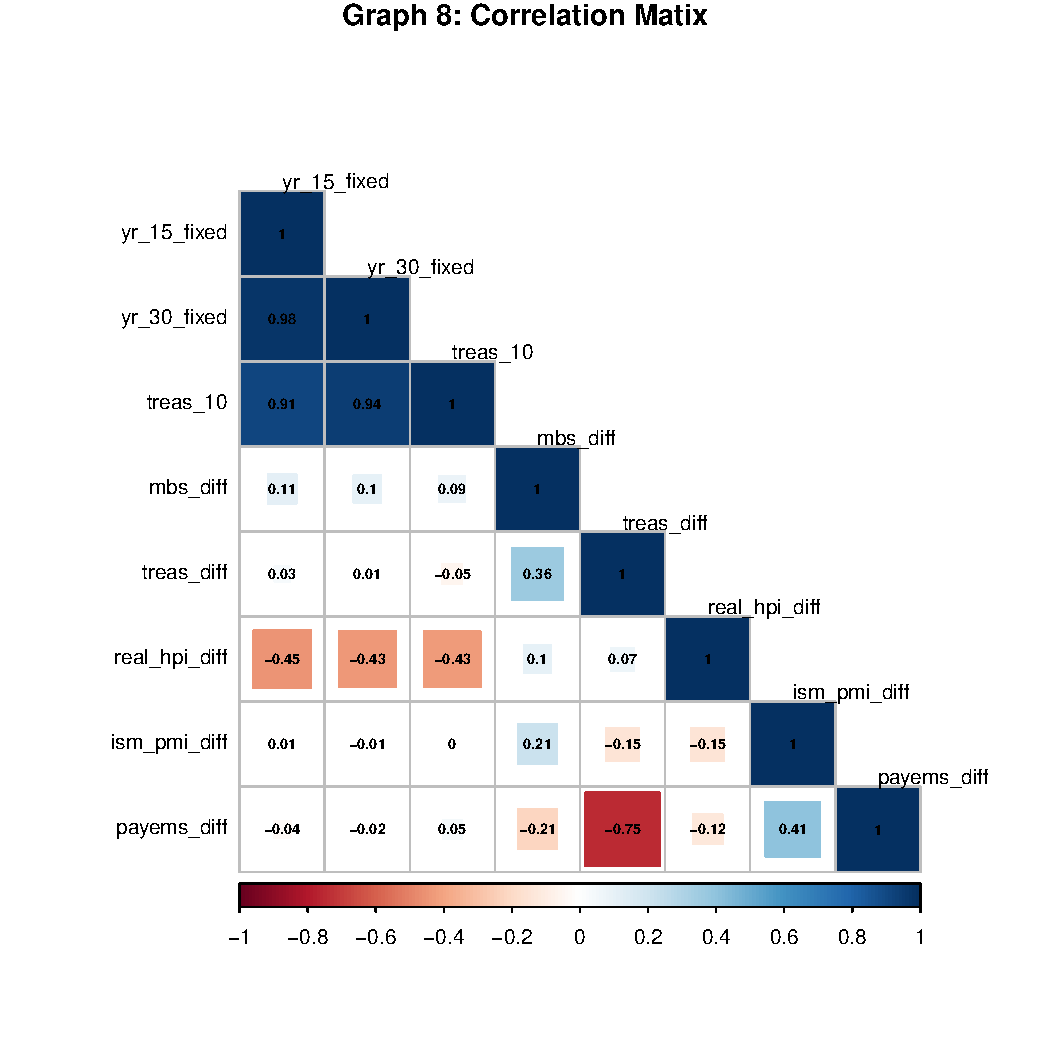
\includegraphics[width=\maxwidth]{figure/unnamed-chunk-8-1} 

\end{knitrout}


\begin{knitrout}
\definecolor{shadecolor}{rgb}{0.969, 0.969, 0.969}\color{fgcolor}
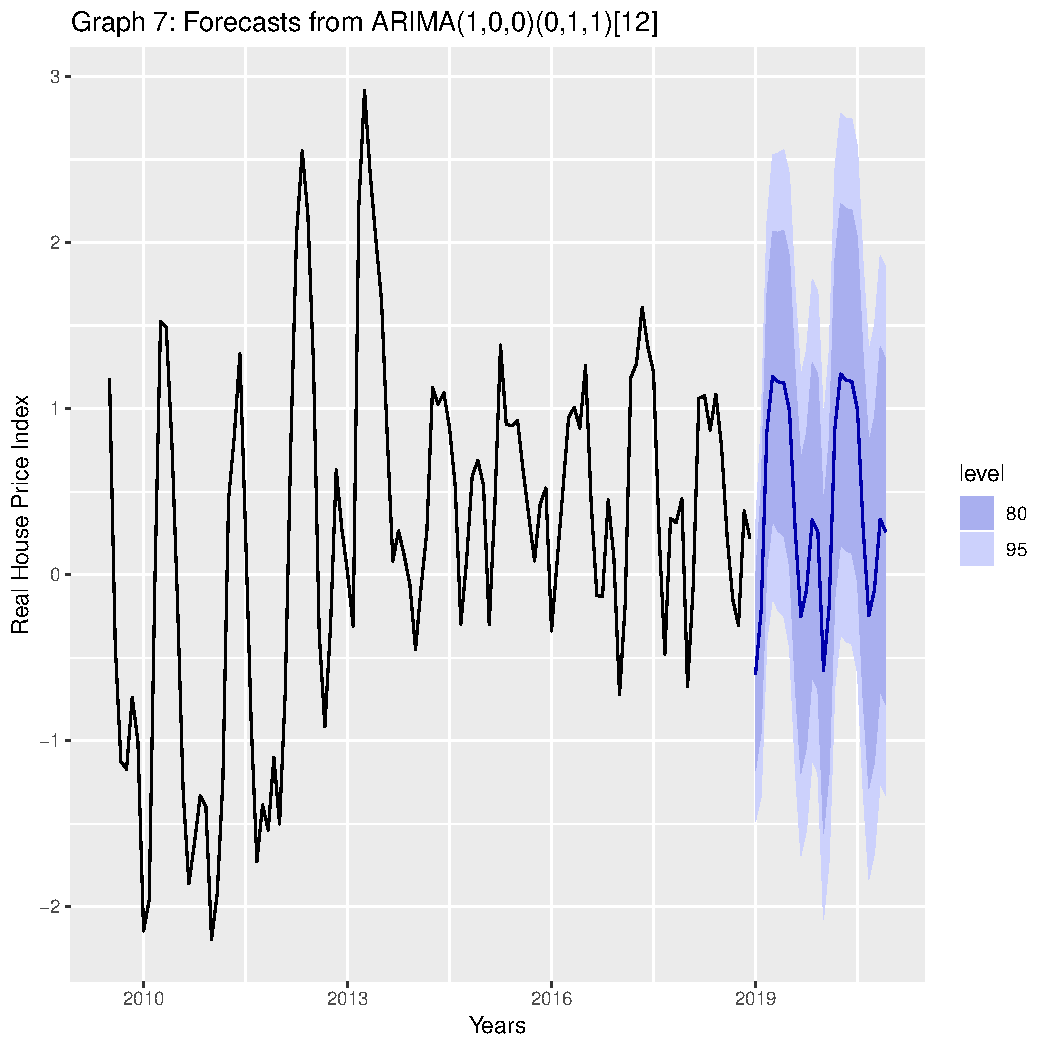
\includegraphics[width=\maxwidth]{figure/unnamed-chunk-9-1} 

\end{knitrout}

\newpage

\begin{knitrout}
\definecolor{shadecolor}{rgb}{0.969, 0.969, 0.969}\color{fgcolor}\begin{kframe}
\begin{verbatim}
## 
## Call:
## tslm(formula = real_hpi_diff ~ mbs_diff + ism_pmi_diff + payems_diff + 
##     treas_10 + yr_30_fixed, data = x5_test_ts)
## 
## Residuals:
##     Min      1Q  Median      3Q     Max 
## -1.9885 -0.8412 -0.0389  0.7222  3.7868 
## 
## Coefficients:
##                Estimate Std. Error t value Pr(>|t|)    
## (Intercept)   3.234e+00  8.988e-01   3.599 0.000435 ***
## mbs_diff      6.547e+00  2.723e+00   2.405 0.017417 *  
## ism_pmi_diff -1.138e-01  5.030e-02  -2.263 0.025112 *  
## payems_diff  -1.088e-06  5.743e-05  -0.019 0.984914    
## treas_10     -2.671e-01  3.451e-01  -0.774 0.440122    
## yr_30_fixed  -5.570e-01  3.983e-01  -1.398 0.164076    
## ---
## Signif. codes:  0 '***' 0.001 '**' 0.01 '*' 0.05 '.' 0.1 ' ' 1
## 
## Residual standard error: 1.046 on 149 degrees of freedom
## Multiple R-squared:  0.2472,	Adjusted R-squared:  0.2219 
## F-statistic: 9.786 on 5 and 149 DF,  p-value: 4.2e-08
\end{verbatim}
\end{kframe}
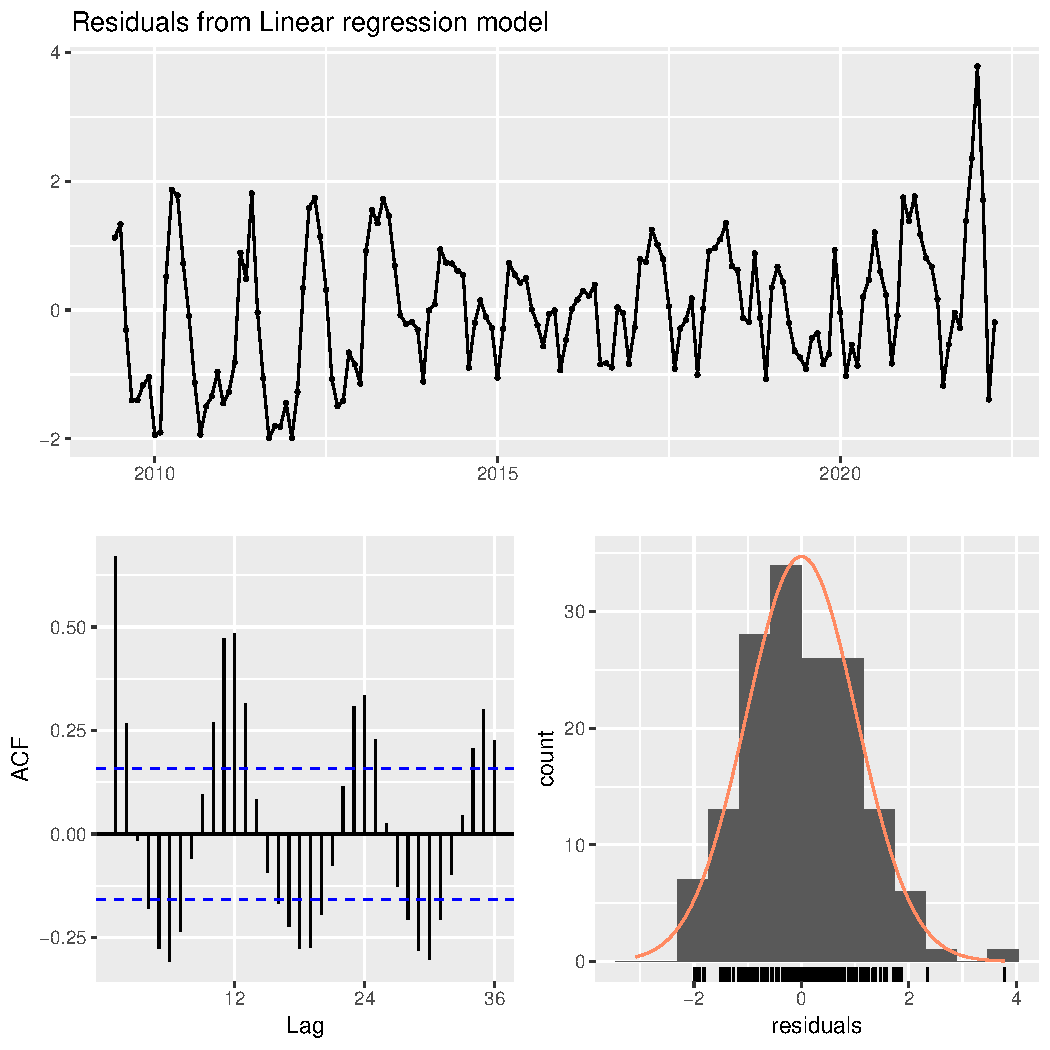
\includegraphics[width=\maxwidth]{figure/Forecasting_Methods-1} 
\begin{kframe}\begin{verbatim}
## 
## 	Breusch-Godfrey test for serial correlation of order up to 24
## 
## data:  Residuals from Linear regression model
## LM test = 107.2, df = 24, p-value = 1.732e-12
## 
## Call:
## tslm(formula = real_hpi_diff ~ treas_diff + ism_pmi_diff + payems_diff + 
##     yr_30_fixed, data = x5_test_ts)
## 
## Residuals:
##     Min      1Q  Median      3Q     Max 
## -2.1234 -0.7345 -0.0588  0.6866  3.9197 
## 
## Coefficients:
##                Estimate Std. Error t value Pr(>|t|)    
## (Intercept)   3.747e+00  5.503e-01   6.809 2.21e-10 ***
## treas_diff   -2.307e-01  3.366e+00  -0.069    0.945    
## ism_pmi_diff -7.009e-02  4.976e-02  -1.409    0.161    
## payems_diff  -5.921e-05  8.341e-05  -0.710    0.479    
## yr_30_fixed  -8.140e-01  1.350e-01  -6.027 1.24e-08 ***
## ---
## Signif. codes:  0 '***' 0.001 '**' 0.01 '*' 0.05 '.' 0.1 ' ' 1
## 
## Residual standard error: 1.064 on 150 degrees of freedom
## Multiple R-squared:  0.2158,	Adjusted R-squared:  0.1949 
## F-statistic: 10.32 on 4 and 150 DF,  p-value: 2.073e-07
\end{verbatim}
\end{kframe}
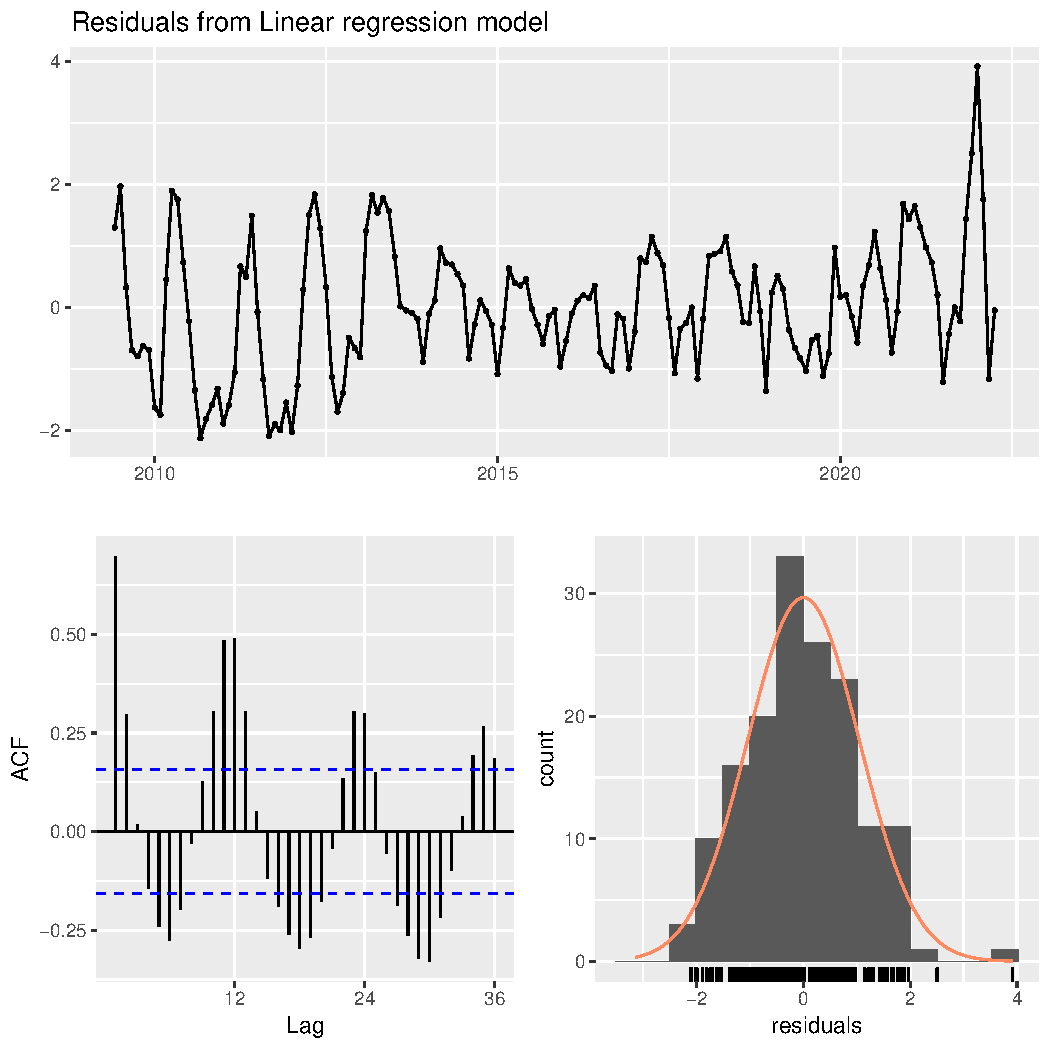
\includegraphics[width=\maxwidth]{figure/Forecasting_Methods-2} 
\begin{kframe}\begin{verbatim}
## 
## 	Breusch-Godfrey test for serial correlation of order up to 24
## 
## data:  Residuals from Linear regression model
## LM test = 109.85, df = 24, p-value = 5.991e-13
## 
## Call:
## tslm(formula = real_hpi_diff ~ treas_diff + ism_pmi_diff + yr_15_fixed + 
##     payems_diff, data = x5_test_ts)
## 
## Residuals:
##     Min      1Q  Median      3Q     Max 
## -2.1714 -0.6647 -0.0832  0.6782  3.8997 
## 
## Coefficients:
##                Estimate Std. Error t value Pr(>|t|)    
## (Intercept)   3.293e+00  4.564e-01   7.214 2.51e-11 ***
## treas_diff   -2.010e-01  3.336e+00  -0.060    0.952    
## ism_pmi_diff -6.226e-02  4.933e-02  -1.262    0.209    
## yr_15_fixed  -8.470e-01  1.344e-01  -6.303 3.08e-09 ***
## payems_diff  -6.846e-05  8.269e-05  -0.828    0.409    
## ---
## Signif. codes:  0 '***' 0.001 '**' 0.01 '*' 0.05 '.' 0.1 ' ' 1
## 
## Residual standard error: 1.054 on 150 degrees of freedom
## Multiple R-squared:  0.2299,	Adjusted R-squared:  0.2094 
## F-statistic: 11.19 on 4 and 150 DF,  p-value: 5.658e-08
\end{verbatim}
\end{kframe}
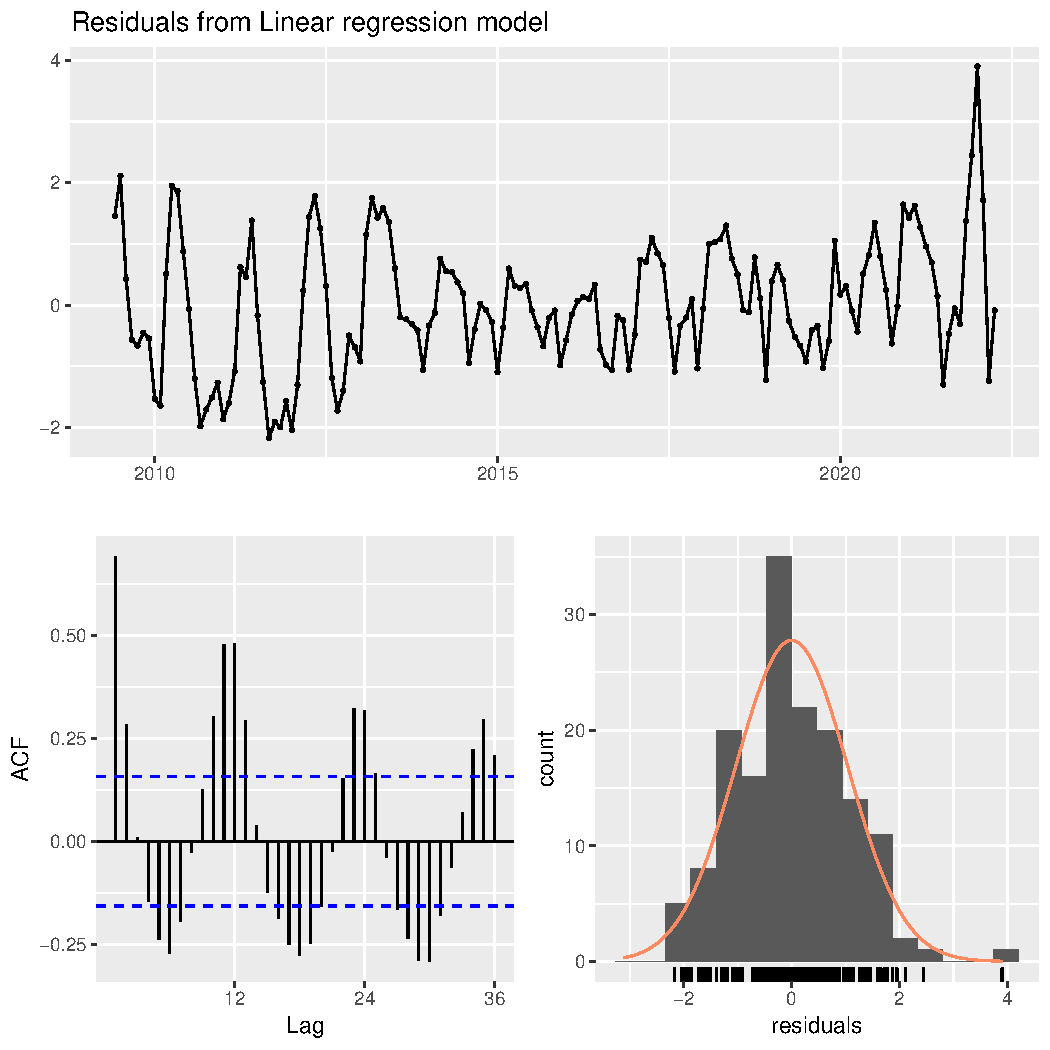
\includegraphics[width=\maxwidth]{figure/Forecasting_Methods-3} 
\begin{kframe}\begin{verbatim}
## 
## 	Breusch-Godfrey test for serial correlation of order up to 24
## 
## data:  Residuals from Linear regression model
## LM test = 108.37, df = 24, p-value = 1.084e-12
\end{verbatim}
\end{kframe}
\end{knitrout}

\begin{knitrout}
\definecolor{shadecolor}{rgb}{0.969, 0.969, 0.969}\color{fgcolor}
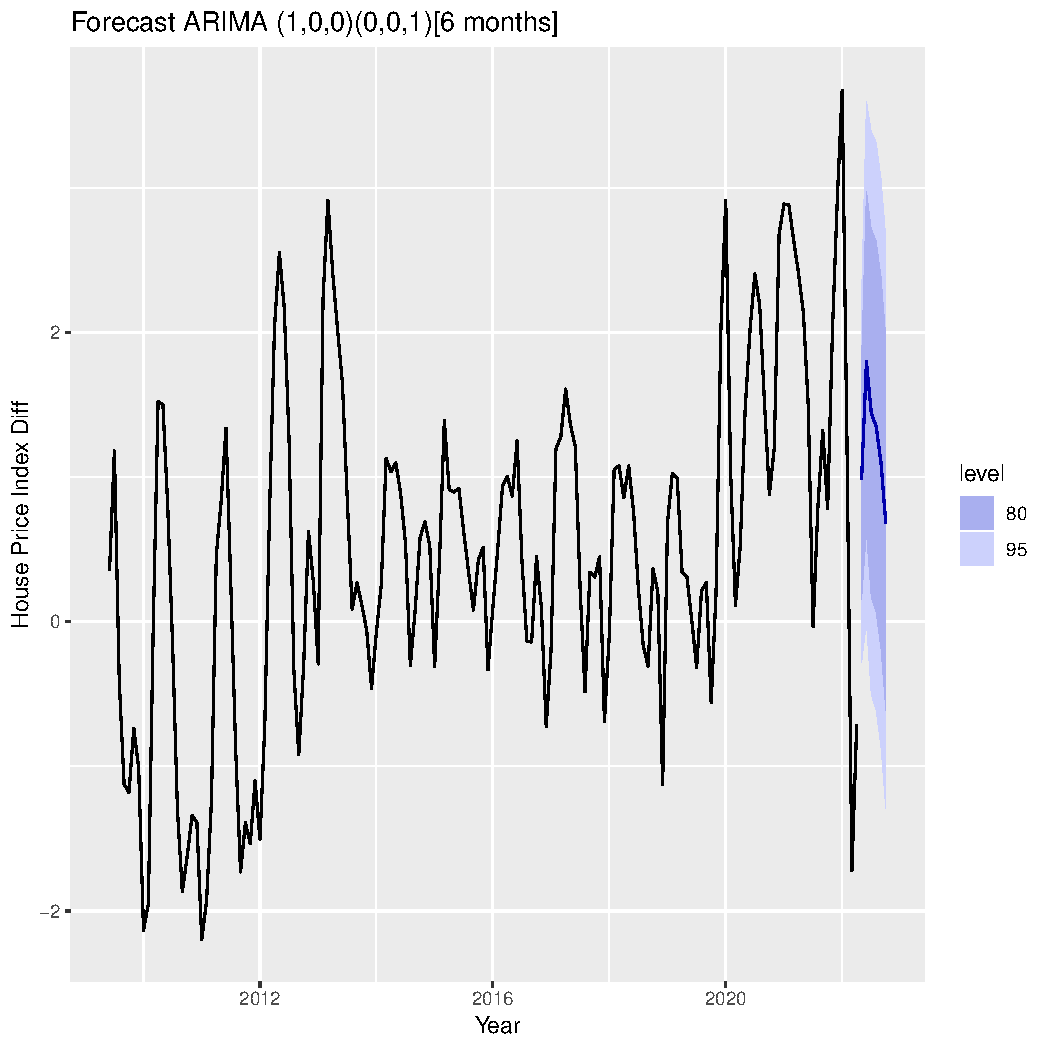
\includegraphics[width=\maxwidth]{figure/unnamed-chunk-10-1} 

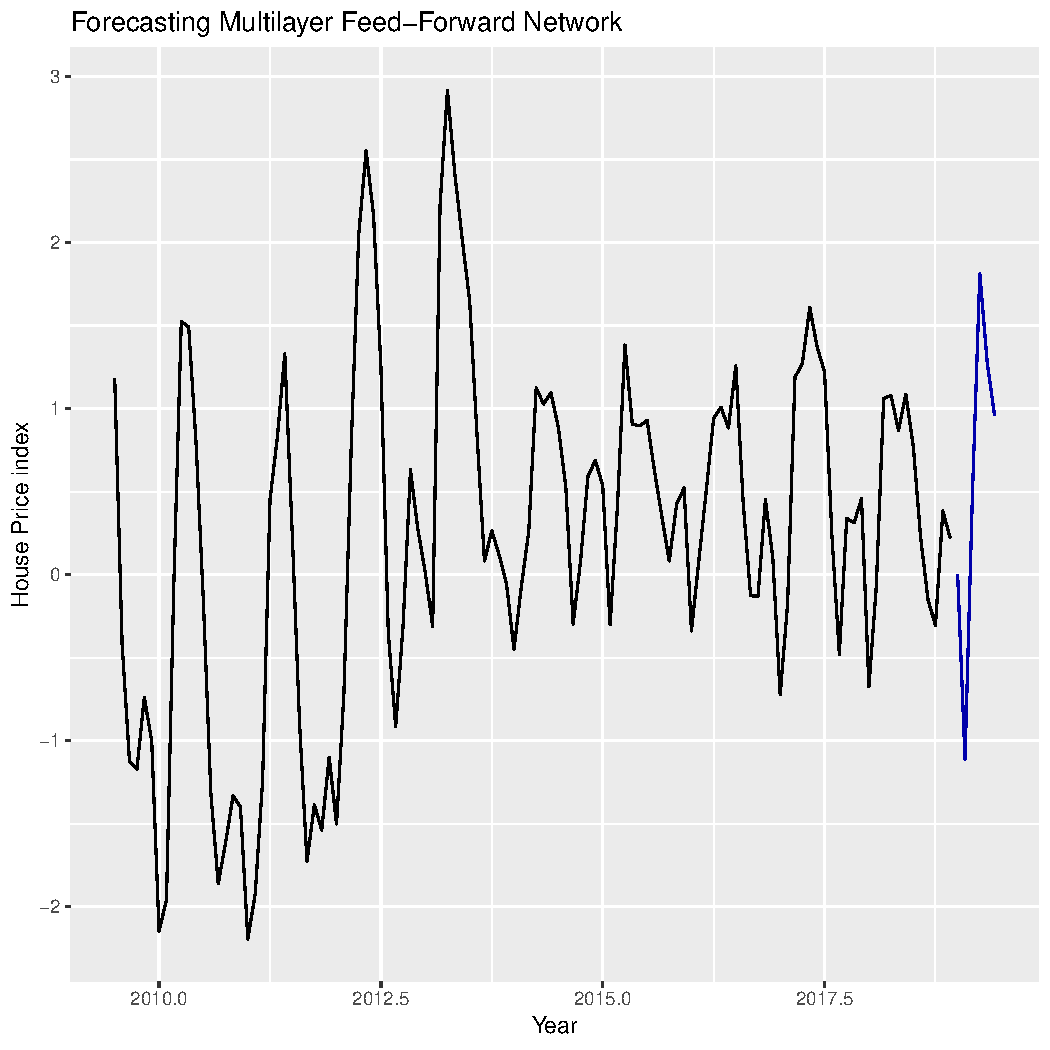
\includegraphics[width=\maxwidth]{figure/unnamed-chunk-10-2} 

\end{knitrout}

\begin{knitrout}
\definecolor{shadecolor}{rgb}{0.969, 0.969, 0.969}\color{fgcolor}\begin{kframe}
\begin{verbatim}
## 
## Call:
## tslm(formula = real_hpi_diff ~ mbs_diff + ism_pmi_diff + payems_diff + 
##     treas_10 + yr_30_fixed, data = train_clean)
## 
## Residuals:
##      Min       1Q   Median       3Q      Max 
## -2.13255 -0.75882 -0.00423  0.68992  1.96011 
## 
## Coefficients:
##                Estimate Std. Error t value Pr(>|t|)   
## (Intercept)   1.2633912  2.2577055   0.560  0.57695   
## mbs_diff      9.1601867  3.4760662   2.635  0.00968 **
## ism_pmi_diff -0.1183327  0.0608136  -1.946  0.05435 . 
## payems_diff   0.0015522  0.0008091   1.918  0.05778 . 
## treas_10     -0.4726571  0.7462915  -0.633  0.52789   
## yr_30_fixed  -0.0495362  0.9513353  -0.052  0.95857   
## ---
## Signif. codes:  0 '***' 0.001 '**' 0.01 '*' 0.05 '.' 0.1 ' ' 1
## 
## Residual standard error: 1.01 on 105 degrees of freedom
## Multiple R-squared:  0.1638,	Adjusted R-squared:  0.124 
## F-statistic: 4.114 on 5 and 105 DF,  p-value: 0.001884
\end{verbatim}
\end{kframe}
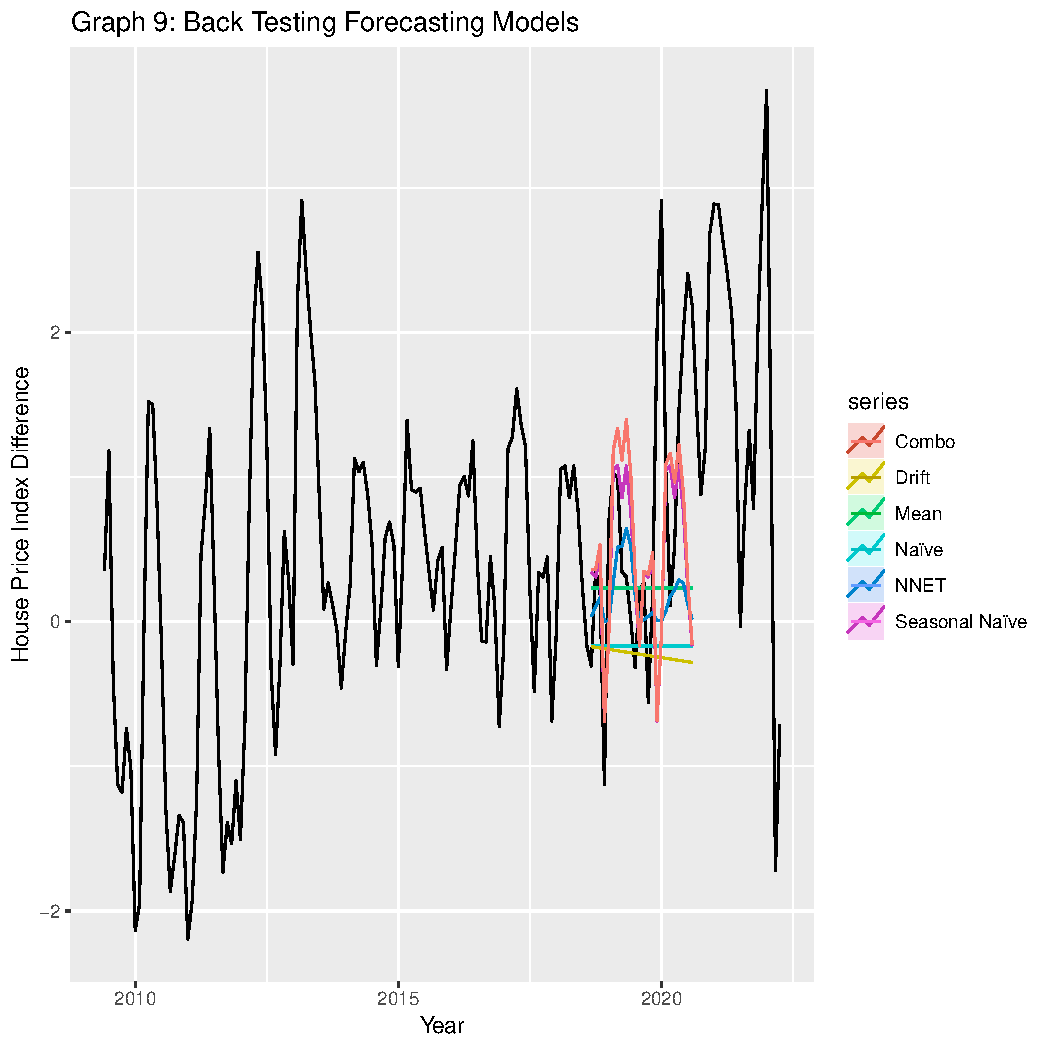
\includegraphics[width=\maxwidth]{figure/unnamed-chunk-11-1} 
\begin{table}[t]

\caption{\label{tab:unnamed-chunk-11}Mean Forecast}
\centering
\fontsize{10}{12}\selectfont
\begin{tabular}{l|r|r|r|r|r|r|r|r}
\hline
  & ME & RMSE & MAE & MPE & MAPE & MASE & ACF1 & Theil's U\\
\hline
Training set & 0.0000000 & 1.074499 & 0.8505951 & 95.09796 & 112.0645 & 1.423644 & 0.7704250 & NA\\
\hline
Test set & 0.4747289 & 1.097606 & 0.7804229 & -17.70224 & 151.2597 & 1.306196 & 0.5514098 & 1.565753\\
\hline
\end{tabular}
\end{table}

\begin{table}[t]

\caption{\label{tab:unnamed-chunk-11}Na�ve Forecast}
\centering
\fontsize{10}{12}\selectfont
\begin{tabular}{l|r|r|r|r|r|r|r|r}
\hline
  & ME & RMSE & MAE & MPE & MAPE & MASE & ACF1 & Theil's U\\
\hline
Training set & -0.0047522 & 0.7302961 & 0.5710356 & -17.05473 & 164.6397 & 0.9557441 & 0.2867814 & NA\\
\hline
Test set & 0.8758972 & 1.3215774 & 1.0125107 & 185.11551 & 185.1155 & 1.6946424 & 0.5514098 & 0.6331836\\
\hline
\end{tabular}
\end{table}

\begin{table}[t]

\caption{\label{tab:unnamed-chunk-11}Seasonal Na�ve Forecast}
\centering
\fontsize{10}{12}\selectfont
\begin{tabular}{l|r|r|r|r|r|r|r|r}
\hline
  & ME & RMSE & MAE & MPE & MAPE & MASE & ACF1 & Theil's U\\
\hline
Training set & 0.0932894 & 0.8162041 & 0.5974775 & 35.03742 & 133.0646 & 1.000000 & 0.6963914 & NA\\
\hline
Test set & 0.2749869 & 1.1792750 & 0.8169461 & -273.56706 & 390.9764 & 1.367325 & 0.4978262 & 1.573682\\
\hline
\end{tabular}
\end{table}

\begin{table}[t]

\caption{\label{tab:unnamed-chunk-11}Drift Forecast}
\centering
\fontsize{10}{12}\selectfont
\begin{tabular}{l|r|r|r|r|r|r|r|r}
\hline
  & ME & RMSE & MAE & MPE & MAPE & MASE & ACF1 & Theil's U\\
\hline
Training set & 0.0000000 & 0.7302807 & 0.570690 & -16.96595 & 164.4944 & 0.9551656 & 0.2867814 & NA\\
\hline
Test set & 0.9352999 & 1.3765463 & 1.060033 & 211.70806 & 211.7081 & 1.7741803 & 0.5631327 & 0.5719166\\
\hline
\end{tabular}
\end{table}

\begin{table}[t]

\caption{\label{tab:unnamed-chunk-11}Neural Net AR Forecast}
\centering
\fontsize{10}{12}\selectfont
\begin{tabular}{l|r|r|r|r|r|r|r|r}
\hline
  & ME & RMSE & MAE & MPE & MAPE & MASE & ACF1 & Theil's U\\
\hline
Training set & 0.0682918 & 0.5819563 & 0.4255376 & 54.23926 & 73.40085 & 0.7122237 & 0.4470948 & NA\\
\hline
Test set & 0.5309625 & 1.1509929 & 0.8362769 & -116.27154 & 263.63416 & 1.3996794 & 0.5697866 & 1.456695\\
\hline
\end{tabular}
\end{table}

\begin{table}[t]

\caption{\label{tab:unnamed-chunk-11}Combination: NNET & SNa�ve}
\centering
\fontsize{10}{12}\selectfont
\begin{tabular}{l|r|r|r|r|r|r|r}
\hline
  & ME & RMSE & MAE & MPE & MAPE & ACF1 & Theil's U\\
\hline
Test set & 0.1866977 & 1.201757 & 0.8717786 & -381.7028 & 499.5252 & 0.5118628 & 1.82764\\
\hline
\end{tabular}
\end{table}


\end{knitrout}

\begin{knitrout}
\definecolor{shadecolor}{rgb}{0.969, 0.969, 0.969}\color{fgcolor}
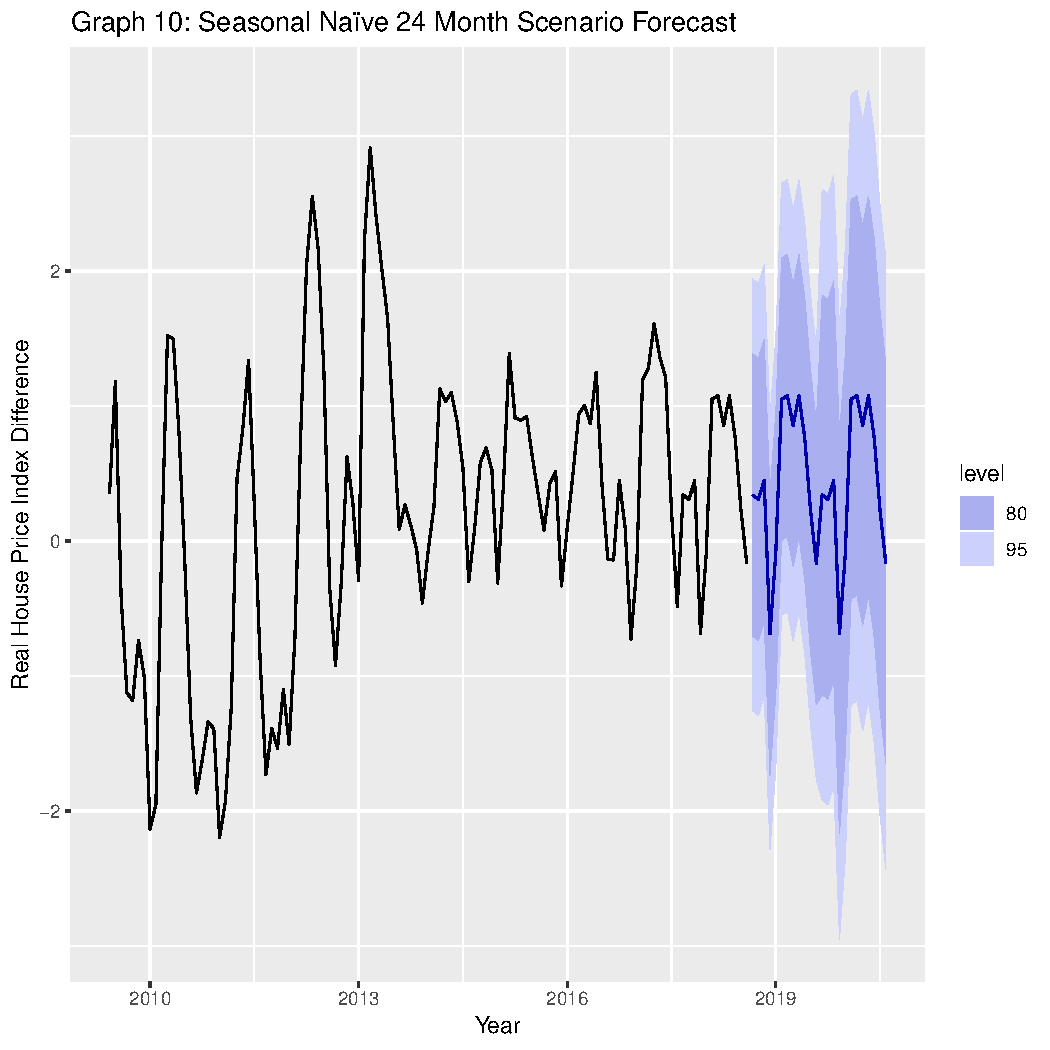
\includegraphics[width=\maxwidth]{figure/unnamed-chunk-12-1} 

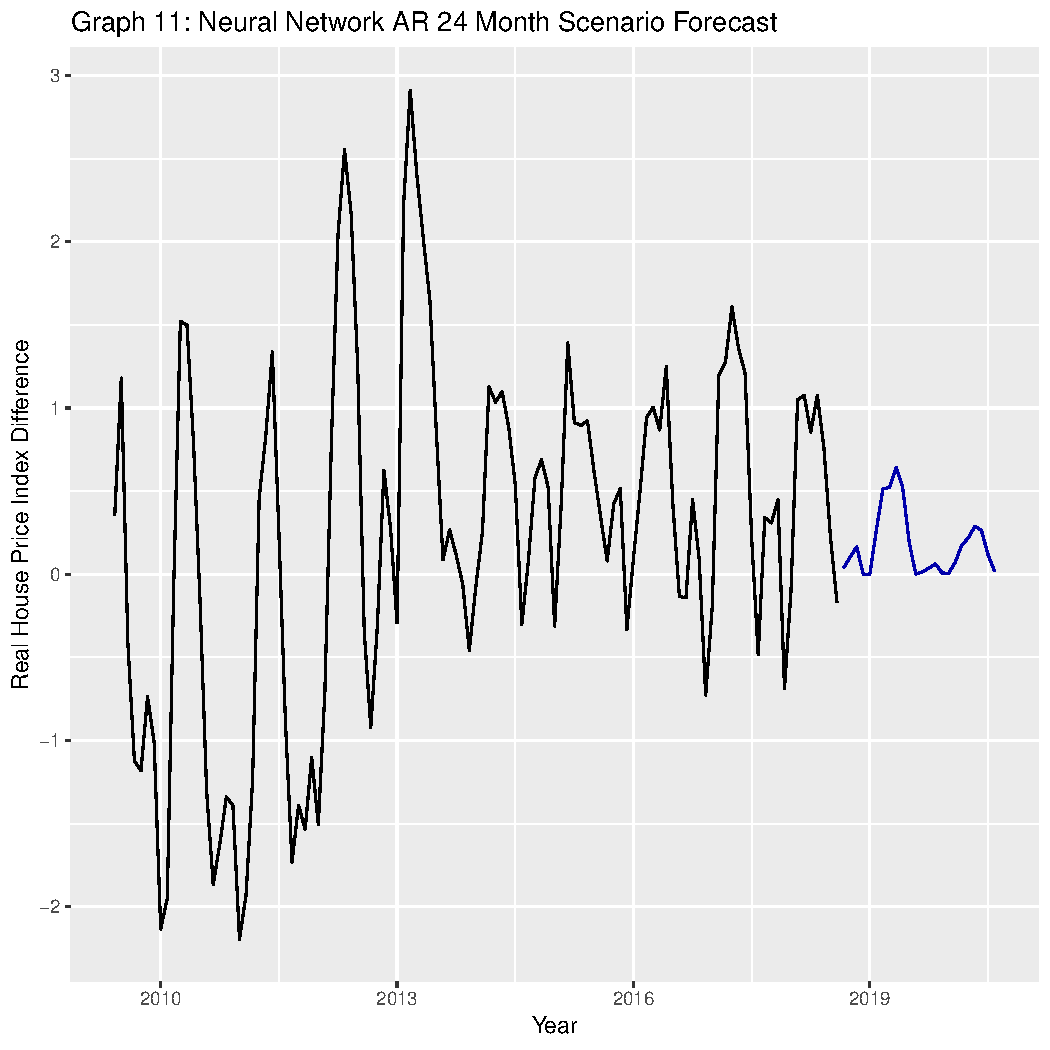
\includegraphics[width=\maxwidth]{figure/unnamed-chunk-12-2} 

\end{knitrout}

\newpage

\begin{singlespace}

\begin{thebibliography}{12}

\bibitem{Cox}
Cox, Jeff (2019). Fed holds rates stable, pledges 'patient' approach, expects 'ample' balance sheet. 
\emph{CNBC}.

\bibitem{Goodman}
Goodman, Laurie and Bing Bai (2017). Normalizing the Federal Reserve's Balance Sheet. The Impact on the 
Mortgage-Backed Securities Market.\emph{The Urban Institute}.

\bibitem{Krishnamurthy}
Krishnamurthy, Arvind and Annette Vissing-Jorgensen, (2013). "The Ins and Outs of LSAPs," Proceedings - 
Economic Policy Symposium - Jackson Hole, \emph{Federal Reserve Bank of Kansas City}.

\bibitem{Kurtz}
Kurtz, Annalyn (2017). 2 Ways the Fed Could Crush the Housing Market Recovery. \emph{Fortune}. 

\bibitem{Geoffrey}
Paulin, Geoffrey (2018). Housing and expenditures: before, during, and after the bubble. \emph{Bureau of Labor Statistics}.

\bibitem{Ng}
Ng, Michael and David Wessel (2017). Housing and expenditures: before, during, and after the bubble. \emph{Brookings Institute}.

\bibitem{Passmore}
Passmore, Wayne and Diana Hancock (2010). Did the Federal Reserve's MBS Purchase Program Lower 
Mortgage Rates? \emph{Board of Governors of the Federal Reserve System}.

\bibitem{Plakandaras}
Plakandaras, Vasilios, Rangan Gupta, Periklis Gogas, and Theophilos Papadimitriou (2017). Forecasting the U.S. Real House Price Index \emph{Democritus University of Thrace, Department of Economics, Cornell University}.

\bibitem{Stroebel}
Stroebel, Johannes and John Taylor (2012). Estimated Impact of the Federal Reserve's Mortgage-Backed 
Securities Purchase Program. \emph{Stanford University}.

\bibitem{Weaver}
Weaver, Jeffrey (2017). The Fed's balance sheet normalization plan. What is the Federal Reserve's plan
and how may it impact investors? \emph{Wells Fargo. Market Insights}. 

\end{thebibliography}
\end{singlespace}


\end{document}

